\documentclass[fr]{../../../../../../eplexam}
\usepackage{listings}
\definecolor{codegreen}{rgb}{0,0.6,0}
\definecolor{codegray}{rgb}{0.5,0.5,0.5}
\definecolor{codepurple}{rgb}{0.58,0,0.82}
\definecolor{backcolour}{rgb}{1.0,1.0,1.0}
\definecolor{codeblue}{rgb}{0,0,0.8}



\lstdefinestyle{mystyle}{
    backgroundcolor=\color{backcolour},   
    commentstyle=\color{codegray},
    keywordstyle=\color{codeblue},
    numberstyle=\tiny\color{codegray},
    stringstyle=\color{codeblue},
    basicstyle=\ttfamily\footnotesize,
    breakatwhitespace=false,         
    breaklines=true,                 
    captionpos=b,                    
    keepspaces=true,                 
    numbers=left,                    
    numbersep=5pt,                  
    showspaces=false,                
    showstringspaces=false,
    showtabs=false,                  
    tabsize=2,
    frame=shadowbox
}
\lstset{style=mystyle}
\lstset{language=Oz}

\hypertitle{}{4}{INFO}{1104}{2021}{Juin}{All}
{Norah Habets \and Thomas Debelle}
{P. Van Roy}

\section{Kernel language}
Translate the following program:
\begin{lstlisting}[escapechar=µ]
local F C in
  C={NewCell 0)
  fun {F A}
    fun {$ B}
      C:=@C+1
      A+B
    end
  end
  {Browse {{F 1} 2}}
end
\end{lstlisting}
into kernel language. Be careful to do a complete translation that uses only kernel language instructions!

\begin{solution}
\begin{lstlisting}[escapechar=µ]
local F C Zero One in
  Zero=0
  One=1
  {NewCell Zero C}
  F=proc{$ A ?R1}
    R1=proc{$ B ?R2}
      local C1 C2 C3 in
        {Exchange C C1 Zero}
        C2=C1+One
        {Exchange C C3 C2}
        R2=A+B
      end
    end
  end
  local F1 F2 Two in
    Two=2
    {F One F1}
    {F1 Two F2}
    {Browse F2}
  end
end
\end{lstlisting}
\end{solution}

\section{Function composition}
Define a function {Compose F G) that takes two one-argument functions F and G and returns their function composition. Give the contextual environment of the function returned by Compose.

\begin{solution}
\begin{lstlisting}[escapechar=µ]
declare
fun {Compose F G}
  fun {$ X}{F {G X}} end
end
\end{lstlisting}
Où E = \{F $\rightarrow$ f, G $\rightarrow$ g\}
\end{solution}

\section{Lambda calculus reduction}
Reduce the expression (SUCC (SUCC 0)) and show itis equivalent to 2. To make your answer easier to understand, only replace a function by its definition When you need it for a reduction step.

\begin{solution}
(SUCC (SUCC 0)) $\longrightarrow$ (SUCC ($\lambda n. \lambda f. \lambda x.f((n f)x) \lambda f( \lambda x.x$)) $\longrightarrow$ (SUCC ($\lambda f. \lambda x.f ((\lambda f (\lambda x.x)f)x)$)) $\longrightarrow$ (SUCC ($\lambda f.(\lambda x.(f.x)$)) $\longrightarrow$ ($\lambda n . \lambda f. \lambda x.f ((n f)x) \lambda f(\lambda x (f x))$) $\longrightarrow$ ($\lambda f. \lambda x.f ((\lambda f (\lambda x(f x))f)x$) $\longrightarrow$ ($\lambda f. \lambda x.f(\lambda x(f x)x)$) $\longrightarrow$ ($\lambda f. \lambda x.f(f x)$) $\longrightarrow$ 2
\end{solution}

\section{Functional programming}
Define the declarative function {Prod F Xs Ys} that has three arguments, a tvvo-argument function F and two lists Xs=[$x_1$ $x_2$ ... $x_n$] and Ys=[$y_1$ $y_2$ ... $y_n$] and returns the list:\\
$[f(x_1, y_1) f(x_1,y_2) ... f(x_1, y_m) f(x_2, y_1) f(x_2, y_2) ... f(x_2, y_m) ... f(x_n, y_1) f(x_n, y_2) ... f(x_n, y_m)]$\\
The number of elements in the returned list is mxn. For example, if Xs=[1 2 3] and Ys=[10 100 1000] and F is multiplication, then the result is [10 100 1000 20 200 2000 30 300 3000). You can define auxiliary functions to simplify your answer. Each recursive function should implement one loop. All functions
should be declarative. Don't worty too much about efficiency, slight inefficiencies will not be penalized.

\begin{solution}
\begin{lstlisting}[escapechar=µ]
declare
fun {Prod F Xs Ys}
  fun {SubProd F X Ys}
    case Ys
    of Y|nil then {F X Y}|nil
    [] Y|Yr then {F X Y}|{SubProd F X Yr}
    end
  end
in
  case Xs
  of X|nil then {SubProd F X Ys}
  [] X|Xr then {Append {SubProd F X Ys} {Prod F Xr Ys}}
  end
end
\end{lstlisting}
\end{solution}

\section{Objects and abstract data types}
In the course we saw two fundamentally different forms of data abstraction, namely objects and abstract data types ADTs and give an example of each.

\begin{solution}
\begin{center}
\begin{minipage}{0.45\linewidth}
Objet: représente à la fois une valeur et un ensemble d'opérations (liés)
\begin{lstlisting}
fun {NewStack}
  C={NewCell nil}
  proc {Push X} C:=X|@C end
  proc {Pop X} S=@C in C:=S.2 X=S.1 end
  proc {IsEmtpy B} B=(@C==nil) end
in
  proc {$ M}
    case M of push(x) then {Push X}
    [] pop(X) then {Pop X}
    [] isEmpty(B) then {IsEmpty B} end
  end
end
\end{lstlisting}
\end{minipage}
%
\begin{minipage}{0.45\linewidth}
Adt: représente un ensemble de valeurs et un ensemble d'opérations (séparés)
\begin{lstlisting}
local Wrap Unwrap in
  {NewWrapper Wrap Unwrap}
  fun {NewStack} 
    {Wrap nil} 
  end
  fun {Push S X} 
    {Wrap X|{Unwrap S}} 
  end
  fun {Pop W X} {Unwrap W} in X=S.1 {Wrap S.2} end
  fun {IsEmpty S} {Unwrap S}==nil end
end
\end{lstlisting}
\end{minipage}
\end{center}
\end{solution}

\section{Exception}
To handle exceptional situations in a program. we add a new concept called exceptions. We introduce two new instructions for exceptions, namely try $<s>_1$ catch $<y>$ then $<s>_2$ end and raise $<x>$ end. For this question, give the semantics Of try and raise by showing their effects on the semantic stack.

\begin{solution}
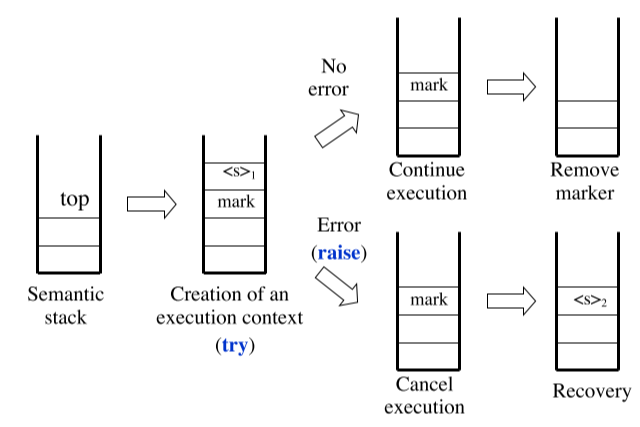
\includegraphics[scale=0.55]{stackException.png}
\end{solution}

\section{The importance of nondeterminism}


\subsection{Definition of nondeterminism}
Define the of nondeterminism in a programming language. Give an example of a program that shows non determinism.

\begin{solution}
Non-déterminisme correspond à la capacité d'un système à faire des  décisions indépendamment du développeur.
\begin{lstlisting}
declare X1 X2
X1=1 X2=2
thread {Browse X1} end
thread {Browse X2} end
\end{lstlisting}
On ne sait pas si X1 va être affiché en premier ou non.
\end{solution}

\subsection{Limitations of deterministic dataflow}
Deterministic dataflow has the strong property that ithas no observable nondeterminism, For this question. give a specification of a client/server application and use this specification to explain Whythe
client/server cannot be written as a deterministic dataflow program. Then define the concept of a port and show in a few lines Of code how to write a client/server by using a port.

\begin{solution}
Sans non-déterminisme observable, le résultat est toujours le même et le choix est pas fait par le scheduler mais par le programmeur.\par 
Or, dans une application client serveur, le résultat dépend de quand on reçoit le message. On reçoit un message, on compile, on répond. Il y a donc d'office du non déterminisme. Le résultat doit être choisi par le scheduler si 2 clients.\par 
Un port est un stream nommé.
\begin{lstlisting}
proc {Server S1 S2}
  case (S1|S2) of (M1|T1)|S2 then
  ... (handle M1)
  {Server T1 S2}
  [] S1|(M2|T2) then
  ... (handle M2)
  {Server S1 T2}
  end
end
\end{lstlisting}
\end{solution}


\section{Erlang support for fault tolerance}

\subsection{Process linking}
An Erlang process is similarto a port Object An important primitive operation to support fault tolerance in Erlang is linking where processes are linked together. For this question. define linking and explain what it does. How does it work when there are more than two processes?

\begin{solution}
Link crée un lien entre 2 processus qui est bidirectionnel dans les 2 sens. Lorsqu'un process s'arrête il envoie le signal "normal" à tous les processus auxquels il est lié, sinon il envoie la cause de son arrêt \textit{anormal}. Les processus qui reçoivent un message "anormal" crash aussi et renvoient le message causant le crash.\par 
Un process peut être configuré pour piéger les signaux de sorte en appelant \textit{process\_flag}(trap\_exit, true)\par 
Un superviseur peut recevoir dans sa mailbox le message sans s'arrêter et prendre des mesures pour restaurer le système. \par 
Ainsi, tous les processus liés au crash en suivant la chaine jusqu'à arriver au superviseur. Si aucun process ne démarre, le programme s'arrête. On peut outrepasser un superviseur avec \textbf{exit(kill, Pid)}.
\end{solution}

\subsection{Supervisor trees}
One of the key concepts in Erlang/OTP to support fault tolerance ts the supervisor tree. Explain what is a supervisor tree. As part of your answer, give two restart strategies and explain how they work. Justify each Strategy with a simple execution scenario.

\begin{solution}
Un arbre de supervision peut redémarrer, modifier ou arrêter un processus qu'il observe (auquel il est lié). Un superviseur, est lui-même supervisé par un autre superviseur, au cas où il échoue. 2 stratégies:
\begin{enumerate}
\item One\_for\_one: quand un des enfants crash, il est simplement redémarré par le superviseur sans que ça n'impacte les autres processus (\textit{ex}: client serveur: pour pas impacter les autres clients si il y a un crash)
\item One\_for\_all: si un des enfants crash, tous les processus liés par le même superviseur sont arrêtés et relancés, même s'ils n'ont aucun problème (\textit{ex}: processus synchronisé: nécessaire quand les processus sont dépendants, pour qu'ils restent synchronisés)
\end{enumerate}
\end{solution}

% Ajouter \nosolution s'il n'y a pas de solution disponible pour cette question

% \nosolution

\end{document}
